%iffalse
\let\negmedspace\undefined
\let\negthickspace\undefined
\documentclass[journal,12pt,onecolumn]{IEEEtran}
\usepackage{cite}
\usepackage{amsmath,amssymb,amsfonts,amsthm}
\usepackage{algorithmic}
\usepackage{graphicx}
\usepackage{textcomp}
\usepackage{xcolor}
\usepackage{txfonts}
\usepackage{listings}
\usepackage{enumitem}
\usepackage{mathtools}
\usepackage{gensymb}
\usepackage{comment}
\usepackage[breaklinks=true]{hyperref}
\usepackage{tkz-euclide} 
\usepackage{listings}
\usepackage{gvv}                                        
%\def\inputGnumericTable{}                                 
\usepackage[latin1]{inputenc}     
\usepackage{xparse}
\usepackage{color}                                            
\usepackage{array}                                            
\usepackage{longtable}                                       
\usepackage{calc}                                             
\usepackage{multirow}
\usepackage{multicol}
\usepackage{hhline}                                           
\usepackage{ifthen}                                           
\usepackage{lscape}
\usepackage{tabularx}
\usepackage{array}
\usepackage{float}
\newtheorem{theorem}{Theorem}[section]
\newtheorem{problem}{Problem}
\newtheorem{proposition}{Proposition}[section]
\newtheorem{lemma}{Lemma}[section]
\newtheorem{corollary}[theorem]{Corollary}
\newtheorem{example}{Example}[section]
\newtheorem{definition}[problem]{Definition}
\newcommand{\BEQA}{\begin{eqnarray}}
\newcommand{\EEQA}{\end{eqnarray}}
\usepackage{float}
\usepackage{listings}
\usepackage{xcolor}
%\newcommand{\define}{\stackrel{\triangle}{=}}
\theoremstyle{remark}
\usepackage{ circuitikz }
%\newtheorem{rem}{Remark}
% Marks the beginning of the document
\begin{document}
\title{}
\author{EE24BTECH11007 - Arnav Makarand Yadnopavit}
\maketitle
\renewcommand{\thefigure}{\theenumi}
\renewcommand{\thetable}{\theenumi}
\parindent 0px Question: Solve the differential equation $y^\prime+y=e^x$ with initial condition $y\brak{0}=1/2$. \\
\solution\\
Theoretical Solution:\\
\begin{align}
    \frac{dy}{dx}+y&=e^x\\
    \frac{dy}{dx} e^x+ye^x&=e^{2x}\\
    d\brak{ye^x}&=e^{2x}dx\\
    \int \frac{d\brak{ye^x}}{dx}&=\int e^{2x}dx\\
    ye^x&=\frac{e^{2x}}{2}+c\\
    y&=\frac{e^x}{2}+ce^{-x}
\end{align}
Substituting values from initial conditions
\begin{align}
    y\brak{0}&=0\\
    \implies c&=0\\
    \therefore y&=\frac{e^x}{2}
\end{align}
The theoretical solution is $f\brak{x}=\frac{e^x}{2}$\\
Computational Solution:\\
We can plot a curve with individual closely spaced points such that
\begin{align}
    y_{n+1}&=y_n+hy^\prime\\
    y_{n+1}&=y_n+h\brak{e^x-y}
\end{align}
\begin{figure}[h]
    \centering
    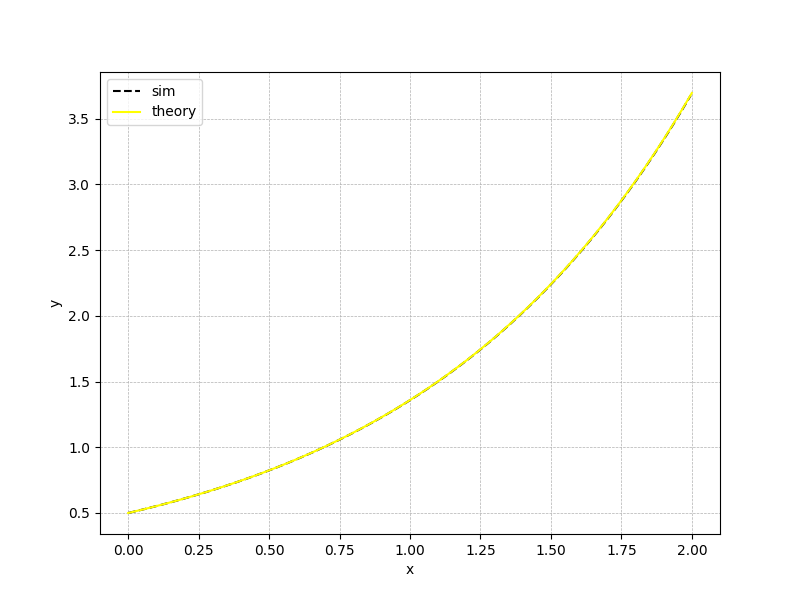
\includegraphics[width=\columnwidth]{figs/fig.png}
 \end{figure}
\end{document}
